\subsection{Optimizations}
\label{sec:seq:optimizations}

\todorev{Last revised on Sat, June 30 at 15:33 by pfac}

While optimizing the sequential code may be important to eliminate possible bottlenecks created by inefficient memory access patterns or poorly written code, most of the optimization work was kept for after the parallelization, as early optimizations might have hampered parallel implementations.
As such, the focus of optimization in the sequential implementation of \polu was on the structures used, which were trivially found to be very inefficient.

As previously stated, the original implementation relied on an AOP approach, but the excessively deep chains of pointers translate into more memory accesses, and consecutively worse performance.

The next two sections describe the two alternative approaches and explain how these improved the application's performance.

\subsubsection{AOS}
% \todo[inline]{Explain the AOS structures and why they should be better than AOP}

The first implemented alternative to AOP was the \textit{Arrays-Of-Structs} approach. Instead of using pointers, structures were created for cells and edges, containing all the data about each. Where pointers existed to link an edge to the adjacent cells, or a cell to its edges, an index is placed. While the dereferencing levels are completely eliminated, using indexes allows any element to hold identifiers which allows direct access to the other elements it needs to interact with, as long as all the data objects are stored in arrays. The maximum representable index is used as the equivalent to \texttt{NULL} pointers (applied, for example, to the right cell of a border edge).
\subsubsection{SOA}
% \todo[inline]{Explain the SOA structures and why they should be better than SOA}

While the AOS approach completely removes the need for dereference, using a \textit{Struct-Of-Arrays} (SOA) approach can be more efficient.

One of the problems with the AOS approach is that when the core functions iterate over one of the arrays, cache lines are being filled with the complete structure of these elements. Yet, neither of the core functions utilizes all the data in that structure, which translates in useless data occupying the cache. This hurts spatial locality\footnote{If a data element is required, it is highly probable adjacent elements will also be required in the near future.}, greatly increasing the chances of accessing a mesh element translating into a RAM access.

The SOA approach solves this problem by placing the data of each element in distinct. As an example, a single array is created to hold the polution level of all the cells. Each data piece is placed in a different array.

This approach allows the core functions to load only the data required for their compuations. The cache lines are now filled only with useful data, and the pieces which are required by the other functions will only be loaded when needed.
\subsubsection{Results}

\todorev{Written on Sat, June 30 at 21:40 by pfac}

To evaluate the impact of the optimizations presented in \cref{sec:321,sec:322}, performance tests were performed with the original and optimized versions.
\Cref{sec:env,sec:method} describe the environmental setup and methodology for the tests performed, respectively.

\Cref{fig:seq:results} shows the results obtained for the three sequential versions.
Both optimized versions show a clear improvement just by not using the several dereference levels. Also, the results show a clear improvement by using SOA over AOS, proving the effectiveness of the optimization.

\begin{figure}[!htp]
	\centering
	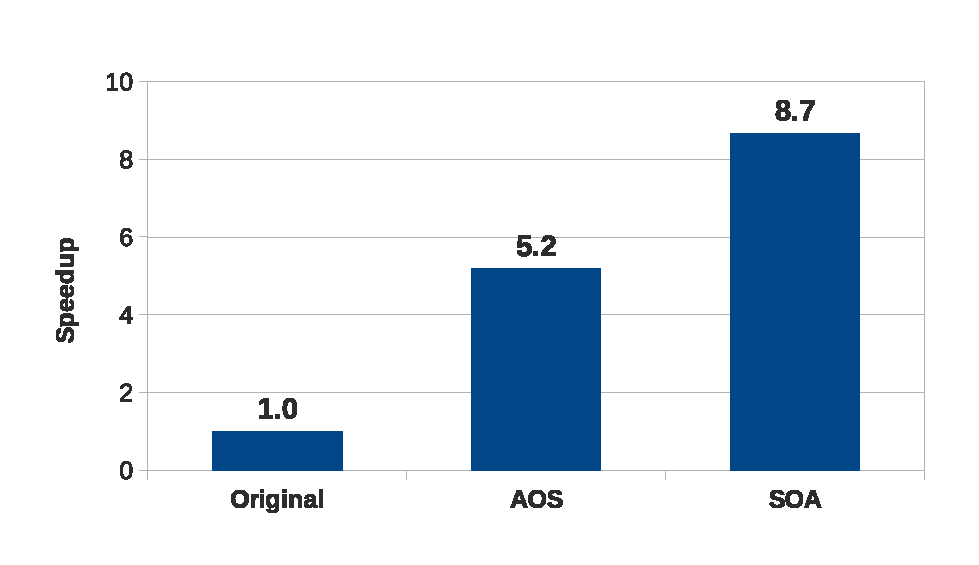
\includegraphics[width=\columnwidth]{images/graph_comparison_seq.eps}
	\caption{Speedup results for the three sequential versions, compared with the original version.}
	\label{fig:seq:results}
\end{figure}